\documentclass[12pt,a4paper]{ctexart}
\usepackage{amsmath,amsthm,amssymb,appendix,bm,graphicx,mathrsfs,abstract,tabularx,xcolor}
\usepackage[colorlinks=true, 
           citecolor=blue,    
           linkcolor=black, 
           pdfborder={0 0 0}]{hyperref}
\usepackage[super,sort&compress]{natbib}
\renewcommand{\bibnumfmt}[1]{[#1]}
\makeatletter
\let\NAT@citex\NAT@citexorig
\makeatother
\usepackage{enumitem}
\usepackage{caption}
\usepackage{geometry}
\usepackage{multirow}
\usepackage{fancyhdr}
\usepackage{booktabs}
\geometry{a4paper,left=3cm,right=2.5cm,top=3cm,bottom=2.5cm}
\usepackage{fontspec}
\setmainfont{Times New Roman}[
    BoldFont=Times New Roman Bold,
    ItalicFont=Times New Roman Italic,
    BoldItalicFont=Times New Roman Bold Italic]
\usepackage{tocloft}
\newfontfamily{\dengxian}{STXihei}
\renewcommand{\cfttoctitlefont}{\hfill\heiti\zihao{3}\bfseries}
\renewcommand{\cftaftertoctitle}{\hfill\mbox{}}
\renewcommand{\cftdot}{.}
\renewcommand{\cftsecleader}{\cftdotfill{\cftdotsep}}
\renewcommand{\cftsubsecleader}{\cftdotfill{\cftdotsep}}
\renewcommand{\cftsubsubsecleader}{\cftdotfill{\cftdotsep}}

\renewcommand{\listfigurename}{图片目录}
\renewcommand{\listtablename}{表格目录}

\renewcommand{\cftloftitlefont}{\hfill\heiti\zihao{3}\bfseries}
\renewcommand{\cftafterloftitle}{\hfill\mbox{}}
\renewcommand{\cftlottitlefont}{\hfill\heiti\zihao{3}\bfseries}
\renewcommand{\cftafterlottitle}{\hfill\mbox{}}

\renewcommand{\cftfigleader}{\cftdotfill{\cftdotsep}}
\renewcommand{\cfttableader}{\cftdotfill{\cftdotsep}}

\renewcommand{\cftfigpresnum}{图}
\renewcommand{\cftfigaftersnum}{}
\setlength{\cftfignumwidth}{3em}

\renewcommand{\cfttabpresnum}{表}
\renewcommand{\cfttabaftersnum}{}
\setlength{\cfttabnumwidth}{3em}

\captionsetup[figure]{labelsep=space}
\captionsetup[table]{labelsep=space} 

\newtheorem{theorem}{定理}[section]
\newtheorem{definition}[theorem]{定义}
\newtheorem{lemma}[theorem]{引理}		
\newtheorem{corollary}[theorem]{推论}
\newtheorem{example}[theorem]{例}
\newtheorem{proposition}[theorem]{命题}
\setcounter{tocdepth}{3} % 显示三级目录
\renewcommand{\contentsname}{\hfill 目录页\hfill} 

\pagestyle{fancy}
\fancyhf{}
\fancyhead[R]{\songti \zihao{-5} 中央民族大学本科生毕业论文(设计)}
\fancyfoot[C]{\thepage}
\renewcommand{\headrulewidth}{0.4pt}
\fancypagestyle{plain}{
  \fancyhf{}
  \fancyhead[R]{\songti \zihao{-5} 中央民族大学本科生毕业论文(设计)}
  \fancyfoot[C]{\thepage}
  \renewcommand{\headrulewidth}{0.4pt}
}

\begin{document}
\thispagestyle{empty}
\vspace*{10pt}
\begin{center}

\includegraphics[width=0.8\textwidth]{muc.png} \\
\vspace{0.5cm}
{\heiti \zihao{-0} 本科毕业论文(设计)} \\
\vspace{1cm}

{
    \renewcommand{\arraystretch}{2.0}
    \begin{tabular}{@{}ll@{}}
        \heiti \zihao{-1}题\hspace{0.5em}目: & 
        \heiti \zihao{-1}\underline{\makebox[16em]{}} \\[0.3cm]
        & \heiti \zihao{2}\underline{\makebox[16em]{\hspace{1em}——}} \\[1cm]
    \end{tabular}

    \begin{tabular}{c}  
        \fangsong \zihao{-3} 姓\hspace{0.8em}名:\underline{\makebox[12em]{your name}} \\[0.5cm]
        \fangsong \zihao{-3} 学\hspace{0.8em}号:\underline{\makebox[12em]{}} \\[0.5cm]
        \fangsong \zihao{-3} 年\hspace{0.8em}级:\underline{\makebox[12em]{21}} \\[0.5cm]
        \fangsong \zihao{-3} 学\hspace{0.8em}院:\underline{\makebox[12em]{information}} \\[0.5cm]
        \fangsong \zihao{-3} 专\hspace{0.8em}业:\underline{\makebox[12em]{communication}} \\[0.5cm]
        \fangsong \zihao{-3} 指导教师:\underline{\makebox[12em]{your teacher}} \\[0.5cm]
    \end{tabular}
}

{\fangsong \zihao{-3}2025年4月7日}
\end{center}


\newpage
\clearpage
\pagenumbering{Roman}
\setcounter{page}{2}

\enlargethispage{\baselineskip}
\vspace*{-\topskip}
\begin{center}
    \heiti \zihao{3} 摘\hspace{1em}要
\end{center}
\vspace{0.1cm}

\zihao{-4} \songti 
\noindent\hspace{2em}论文的摘要是对论文研究内容和成果的高度概括。摘要应对论文所研究的问题及其研究目的进行描述,对研究方法和过程进行简单介绍,对研究成果和所得结论进行概括。
    
\noindent\hspace{2em}摘要应具有独立性和自明性,其内容应包含与论文全文同等量的主要信息。使读者即使不阅读全文,通过摘要就能了解论文的总体内容和主要成果。论文摘要的书写应力求精确、简明。
    
\noindent\hspace{2em}关键词是为了文献标引工作、用以表示全文主要内容信息的单词或术语。关键词不超过5个,每个关键词中间用分号分隔。
    
\vspace{1em}
\noindent{\heiti 关键词:}\songti 关键词1;关键词2;关键词3;关键词4;关键词5

\newpage
\enlargethispage{\baselineskip}
\vspace*{-\topskip}
\begin{center}
    \heiti \zihao{3} Abstract
\end{center}
\vspace{0.1cm}

\fontfamily{ptm}\selectfont
\zihao{-4} 
\noindent\hspace{2em}An abstract of a dissertation is a summary and extraction of research work and contributions. Included in an abstract should be description of research topic and research objective, brief introduction to methodology and research process, and summary of conclusion and contributions of the research.

\noindent\hspace{2em}An abstract should be characterized by independence and clarity and carry identical information with the dissertation. It should be such that the general idea and major contributions of the dissertation are conveyed without reading the dissertation. An abstract should be concise and to the point.

\noindent\hspace{2em}Keywords are terms used in a dissertation for indexing, reflecting core information of the dissertation. An abstract may contain a maximum of 5 keywords, with semi-colons used in between to separate one another.

\vspace{1em}
\noindent{\sffamily\fontseries{b}\selectfont Key words:}~keyword 1;~keyword 2;~keyword 3;~keyword 4;~keyword 5

\fontfamily{\familydefault}\selectfont 

\newpage
\setcounter{page}{4}
\enlargethispage{\baselineskip}
\vspace*{-\topskip}
\addcontentsline{toc}{section}{目录页}
\tableofcontents
\thispagestyle{fancy}

\newpage
\listoffigures
\thispagestyle{fancy}

\newpage
\listoftables
\thispagestyle{fancy}

\newpage
\section*{主要符号说明}
\thispagestyle{fancy}
\begin{description}[leftmargin=4em,itemsep=0.5\baselineskip]
    \item[$f$] 焦距——镜头光学中心到成像平面的距离
    \item[$\delta$] 示例说明文字(请替换为实际含义)
\end{description}

\newpage
\setcounter{page}{1}
\pagenumbering{arabic}
\section{绪论}
\subsection{关于此模板}
本模版主要参考《校发-2023-117-中央民族大学关于印发〈中央民族大学本科毕业论文(设计)工作管理办法〉的通知(1)》、《〈中央民族大学本科生毕业论文(设计)的规定〉》、《中央民族大学毕业设计(论文)格式基本要求》等。

各个模版有些细微差异,整合过后得到此模版。

\subsection{补充说明}
这是一个来自民间的模版,已经交由电子信息大类的负责老师过审。不过有些具体细节可能没考虑到,遇到格式问题时,建议咨询毕设导师的意见。
\subsubsection{更细节的说明}
几乎每一个需要特别注意的样式都在样式库里创建了对应模版,大家点击对应的样式窗格就可以直接使用。
\subsubsection{同样是更细节的说明}
这是一个三级标题,建议标题层级不要超过三级。

\newpage
\section{图表示例}
\subsection{插图}
毕业论文的插图应与文字紧密配合,文图相符,技术内容正确。选图要力求精练,线条要匀称,图面要整洁美观,每幅插图应有图序和图题(五号宋体加黑),全文插图可以统一编序,也可以逐章单独编序,不管采用哪种方式,图序必须连续,不得重复或跳缺。由若干分图组成的插图,分图用 a、b、c……标序,分图的图名以及图中各种代号的意义,以图注形式写在图题下方,先写分图名,另起行后写代号的意义。图应在描纸或洁白纸上用墨线绘成,或用计算机绘图,电气图或机械图应符合相应的国家标准的要求。坐标图:横纵坐标必须标注量、单位,坐标名置于图的下方居中,五号宋体加黑。

如图1所示,这是一张插图
\begin{figure}[h]
\centering
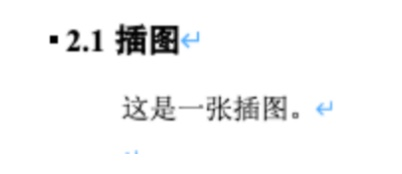
\includegraphics[width=0.6\textwidth]{1.png}
\caption{这是一张插图}
\label{fig:example}
\end{figure}

注意:可以选择使用PPT作图,并导出矢量图(建议自行搜索“论文图片格式指南”)。

\subsection{表格}
这是表格
\begin{table}[h]
    \centering
    \caption{这是一个三线表}
    \begin{tabular}{ll}
        \toprule
        文件名 & 描述 \\
        \midrule
        main.py & 主函数 \\
        xxx.py & xxx \\
        xxxx.py & xxxx \\
        \bottomrule
    \end{tabular}
\end{table}

\section{数学符号和公式}
\subsection{数学符号}
中文论文的数学符号默认遵循 GB/T 3102.11—1993《物理科学和技术中使用的数学符号》。毕业论文中的测量、统计数据一律用阿拉伯数字,如 5.25MeV 等。在叙述较小的数量时,一般不宜用阿拉伯数字
\subsection{公式}
于数学公式,应当使用数学“公式编辑器” 来输入。例如:

\[
(x+a)^n = x = \frac{-b \pm \sqrt{b^2 - 4ac}}{2a} \sum_{k=0}^n \binom{n}{k} x^k a^{n - k} \quad \#(1)
\]

公式应另起一行写在稿纸中央,一行写不完的长公式,最好在等号处转行,如做不到这点,在数学符号(如“+”、“-”号)处转行,数学符号应写在转行后的行首。公式的编号用圆括号括起放在公式右边行末,在公式和编号之间不加虚线,公式可按全文统一编序号,也可以逐章编序,公式序号必须连续,不得重复或跳缺。重复引用的公式不得另编新序号。公式中分数的横分线要写清楚,特别是连分数(即分子和分母也出现分数时),更要注意分线的长短,并将主要分线和等号对齐。在叙述中也可将分数的分子和分母平列在一行,用斜线分开表述。

\[
f(x) = a_0 + \sum_{n=1}^{\infty} \left( a_n \cos \frac{n \pi x}{L} + b_n \sin \frac{n \pi x}{L} \right) \quad \#(2)
\]

如果你的公式显示不全,尝试调整行间距,改为“单倍间距”就可以了。

\newpage
\section{参考文献}
\subsection{参考文献格式}
引用示例:二次铣削\cite{ref1},由文献\cite{ref2,ref3}可知...

本用文献标示应置于所引内容最末句的右上角,用五号TimesNewRoman字体。所引文献编号用阿拉伯数字置于中括号“[]”中,以上标的形式标示。如“二次铣削[1]”。当提及的参考文献为文中直接说明时,其序号应该用五号宋体与正文排齐,如“由文献[8,10~14]可知”。不得将引用文献标示置于各级标题处。
\subsection{格式示例}
1.专著

主要责任者.题名:其他题名信息[文献类型标志].其他责任者.版本项.出版地:出版者,出版年:引文页码[引用日期].获取和访问路径.

示例:

[1]余敏.出版集团研究[M].北京:中国书籍出版社,2001:179-193.

2.专著中的析出文献

析出文献主要责任者.析出文献题名[文献类型标志].析出文献其他责任者//专著主要责任者.专著题名:其他题名信息.版本项.出版地:出版者,出版年:析出文献的页码[引用日期].获取和访问路径.

示例:

[2]程根伟.1998 年长江洪水的成因与减灾对策[M]//许厚泽,赵其国.长江流域洪涝灾害与科技对策.北京:科学出版社,1999:32-36.

3.连续出版物

主要责任者,题名:其他题名信息[文献类型标志].年,卷(期)-年,卷(期).出版地:出版者,出版年[引用日期].获取和访问路径.

示例:

[3]中国图书馆学会.图书馆学通讯[J].1957(l)-1990(4).北京:北京图书馆,1957-1990.

4. 连续出版物中的析出文献

析出文献主要责任者.析出文献题名[文献类型标志].连续出版物题名:其他题名信息,年,卷(期):页码[引用日期].获取和访问路径.

示例:

[4]李晓东,张庆红,叶瑾琳.气候学研究的若干理论问题[J].北京大学学报:自然科学版,1999,35(1):101-106.

5. 专利文献

专利申请者或所有者.专利题名:专利国别,专利号[文献类型标志].公告日期或公开日期[引用日期].获取和访问路径.

示例:

[5]姜锡洲.一种温热外敷药制备方案:中国,88105607,3[P].1989-07-26.

6.电子文献

主要责任者.题名:其他题名信息[文献类型标志/文献载体标志].出版地:出版者,出版年(更新或修改日期)[引用日期].获取和访问路径.

示例:

[6]	HOPKINSONA.UNIMARCandmetadsta:DublinCore[EB/OL].[1999-12-08].http://www.ifla.org/IV/ifla64/138-161e.htm.
\subsection{文献管理提示}
如果你见过下面这个工具,应该知道我要说什么了。

\begin{figure}[h]
    \centering
    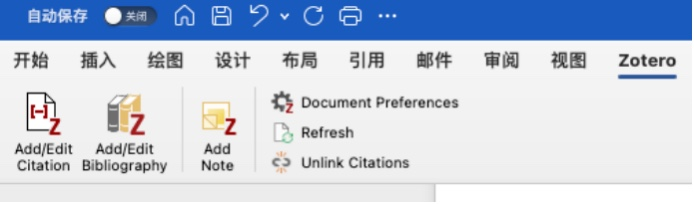
\includegraphics[width=0.6\textwidth]{2.png}
    \caption{zotero文献管理}
    \label{fig:zotero}
    \end{figure}

是的,可以通过zotero进行统一的文献管理,可以上网搜索具体操作,这里不展开。如果觉得配置过程麻烦,也可以参考上面关于文献格式的内容,只要能按照文献格式书写即可。

\newpage
\begin{thebibliography}{99}
    \bibitem{ref1}孟悦. 两千年:女性作为历史的盲点. 上海文论, 1989(2): 18
    \bibitem{ref2}朱传礼. 高等学校毕业设计(论文)指导手册. 高等教育出版社,2001:25
    \bibitem{ref3}朱传礼. 高等学校毕业设计(论文)指导手册. 高等教育出版社,2001:500
    \bibitem{ref4}夏敬华. 企业流程中的常见问题. http://www.amteam.org/bp.asp[EB/OL], 2003年8月9日访问
\end{thebibliography}

\newpage
\begin{appendices}
	\renewcommand{\thesection}{\Alph{section}}
    \captionsetup[table]{labelformat=empty,list=no} % 添加这一行
	\section{附录}
	附录主要列入正文内容过分冗长、或重复性的内容,或者提供查阅方便所需的辅助性表格、计算程序及说明等,如没有相关内容则本部分可以略去。以下是一个附录实例:

    \begin{table}[h]
    \centering
    \caption{附录1 历史纪年对照表 (公元1840--1949年)}
    \begin{tabular}{|c|c|c|c|c|}
    \hline
    公元 & 中国年号 & 干支 & 日本年号 & 伪满年号 \\
    \hline
    1840 & 道光20年 & 庚子鼠 & 天保11年 & 皇纪2500年 \\
    \hline
    1841 & 道光21年 & 辛丑牛 & 天保12年 & 皇纪2501年 \\
    \hline
    1842 & 道光22年 & 壬寅虎 & 天保13年 & 皇纪2502年 \\
    \hline
    1843 & 道光23年 & 癸卯兔 & 天保14年 & 皇纪2503年 \\
    \hline
    1844 & 道光24年 & 甲辰龙 & 弘化元年 & 皇纪2504年 \\
    \hline
    1845 & 道光25年 & 乙巳蛇 & 弘化1年 & 皇纪2505年 \\
    \hline
    1846 & 道光26年 & 丙午马 & 弘化2年 & 皇纪2506年 \\
    \hline
    1847 & 道光27年 & 丁未羊 & 弘化3年 & 皇纪2507年 \\
    \hline
    1848 & 道光28年 & 戊申猴 & 嘉永元年 & 皇纪2508年 \\
    \hline
    \end{tabular}
    \end{table}

\end{appendices}

\newpage
\section*{致谢}
\addcontentsline{toc}{section}{致谢}
谢辞应以简短的文字对课题研究与论文撰写过程中曾直接给予帮助的人员(例如指导教师、答疑教师及其他人员)表示自己的谢意,这不仅是一种礼貌,也是对他人劳动的尊重,是治学者应当遵循的学术规范。

感谢MUC。感谢信息工程学院。电子信息大类无敌!

此模版由人工创作,可能存在部分问题

\end{document}
